\section*{Prescribed motion}
First we intend to test if the fluid equation with and without mapping will respond to a given structural motion. To do this we look at a rectangular mesh (height = 1, width = 2) with a given structural velocity (w0,0) on the left inlet.
\subsection*{Mesh move}
First we have the boundary conditions for w: \\
$ w = (w0,0)$ on the inlet and $w = (0,0)$ on the outlet 
We first solve the laplace equation with w.
$$\Delta t\cdot (\nabla w, \nabla \psi)_{\mathcal{F}} $$
This gives us a w that we use to solve the fluid problem:
$$\rho_f \big( \frac{\partial u}{\partial t} + (\nabla u)(u-w) , \phi\big)_{\mathcal{F}} + (\sigma_f ,\nabla \phi )_{\mathcal{F}} = 0  $$
$$\big( \nabla \cdot u ,\gamma \big)_{\mathcal{F}} = 0 $$
With boundary conditions $u = (w_0,0)$ on the inlet. "Do nothing" on the oulet. And we set $u = (w_x, w_y)$ from the computed w on the top and bottom.
After the fluid is computed we take the calculated w and times it by $\Delta t$ to get the displacement. This is then used to move the mesh. Then we do the calculations with the new mesh, and this process continues.
\subsubsection{Fenics code}
\begin{lstlisting}[frame=single]
# laplace d = 0
F2 =  k*(inner(grad(w), grad(psi))*dx \\
    - inner(grad(w)*n, psi)*ds)

# Fluid variational form
F1 = rho_f*((1.0/k)*inner(u - u0, phi) \
    + inner(dot((u - w_), grad(u)), phi))*dx \
    + inner(sigma_fluid(p, u), grad(phi))*dx \
    - inner(div(u), gamma)*dx\
    - inner(sigma_fluid(p,u)*n, phi)*ds
\end{lstlisting}
The fluid velocity boundary is set in this fashion:
\begin{lstlisting}[frame=single]

# Fluid velocity conditions
class U_bc(Expression):
    def init(self,w):
        self.w = w
    def eval(self,value,x):
        #x_value, y_value = self.w.vector()[[x[0], x[1]]]
        x_value, y_value = self.w(x)
        value[0] = x_value
        value[1] = y_value
    def value_shape(self):
        return (2,)
      
# instance of the class U_bc      
u_bc = U_bc(degree=2)

while t <= T:
    print "Time: ",t
    inlet.t = t
    solve(lhs(F2)==rhs(F2), w_, bcs_w)
    u_bc.init(w_)

    solve(F1==0, up_, bcs_u,solver_parameters={"newton_solver": \
    {"relative_tolerance": 1E-8,"absolute_tolerance":1E-8,"maximum_iterations":100,"relaxation_parameter":1.0}})
    u,p = up_.split(True)
    plot(u)#, interactive=True,mode="displacement")

    flux.append(assemble(dot(u,n)*ds(3)))
    u0.assign(u)

    u_file << u
    #p_file << p
    #w_file << w_

    # To see the mesh move with a give initial w
    w_.vector()[:] *= float(k) # gives displacement to be used in ALE.move(w_)
    ALE.move(mesh,w_)
    mesh.bounding_box_tree().build(mesh)
    #plot(mesh)#,interactive = True)

    t += dt
\end{lstlisting}


\subsection*{Reference mapping}
With the reference frame of mind. We solve the problem in a similar fashion as before but with a the mappings in the fluid equation:

\begin{lstlisting}[frame=single]
F1 = J_*rho_f*((1.0/k)*inner(u - u0, phi) \
    + inner(dot(inv(F_)*(u - w_), grad(u)), phi))*dx \
    + inner(J_*sigma_fluid(p, u)*inv(F_.T), grad(phi))*dx \
    - inner(div(J_*inv(F_.T)*u), gamma)*dx\
    - inner(J_*sigma_fluid(p,u)*inv(F_.T)*n, phi)*ds
\end{lstlisting}

\subsection*{Results}

Reference:\\
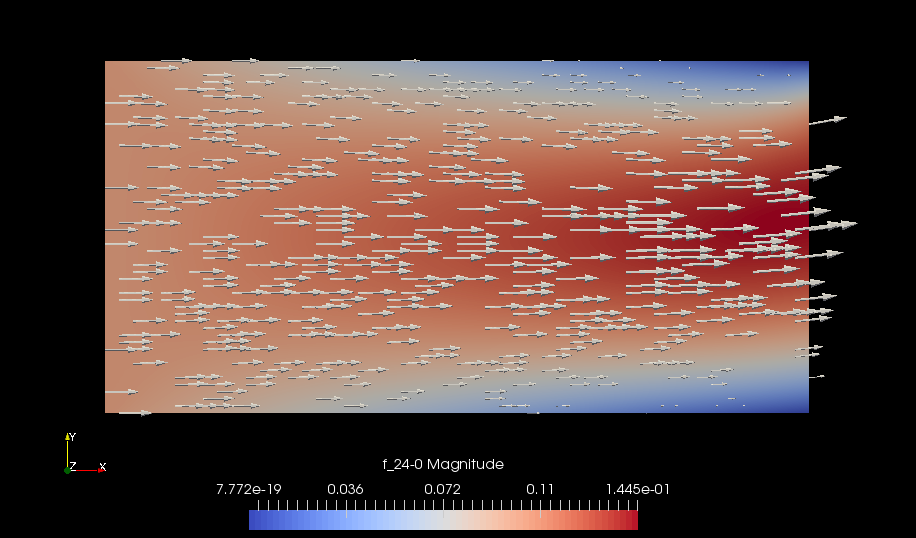
\includegraphics[scale=0.4]{ALE_vector_plot.png}
Moving mesh:\\
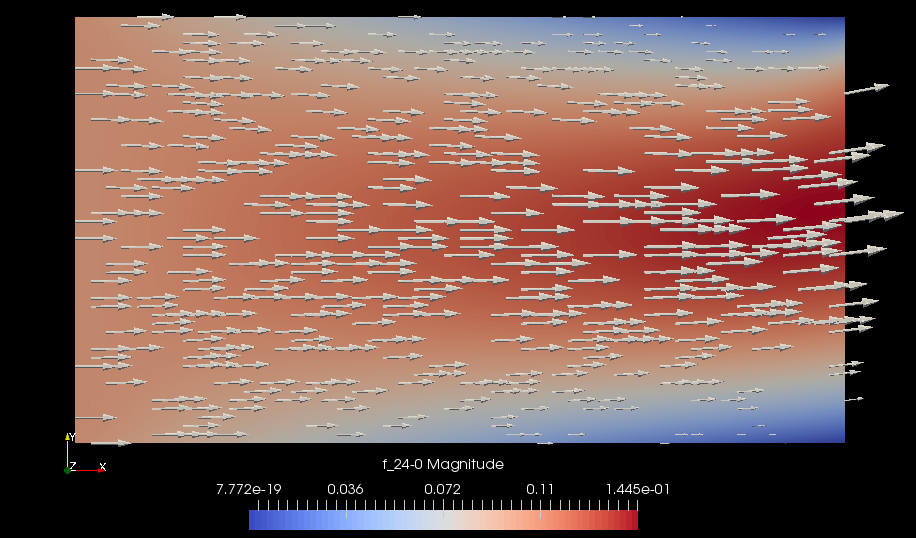
\includegraphics[scale=0.4]{E_vector_plot.png}
Reference:\\
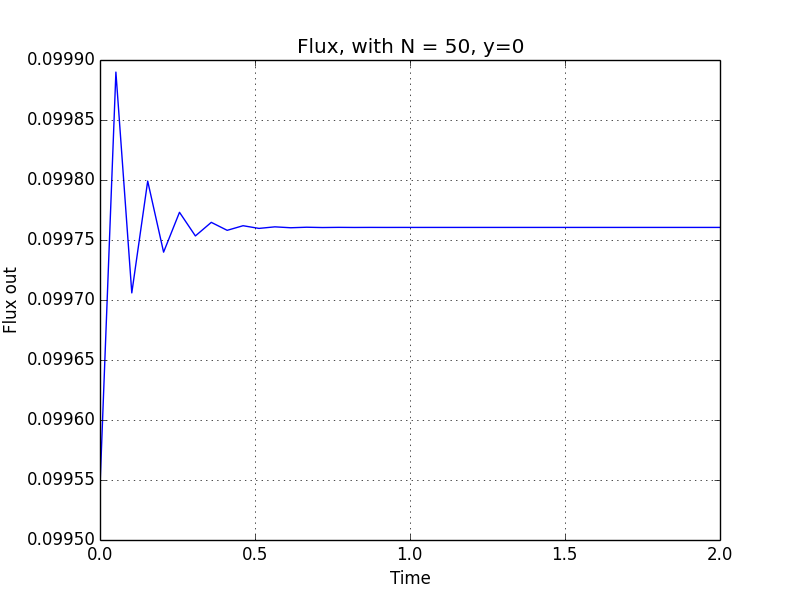
\includegraphics[scale=0.4]{FluxPlot_ALE_N_50_dt_005.png}
Moving mesh:\\
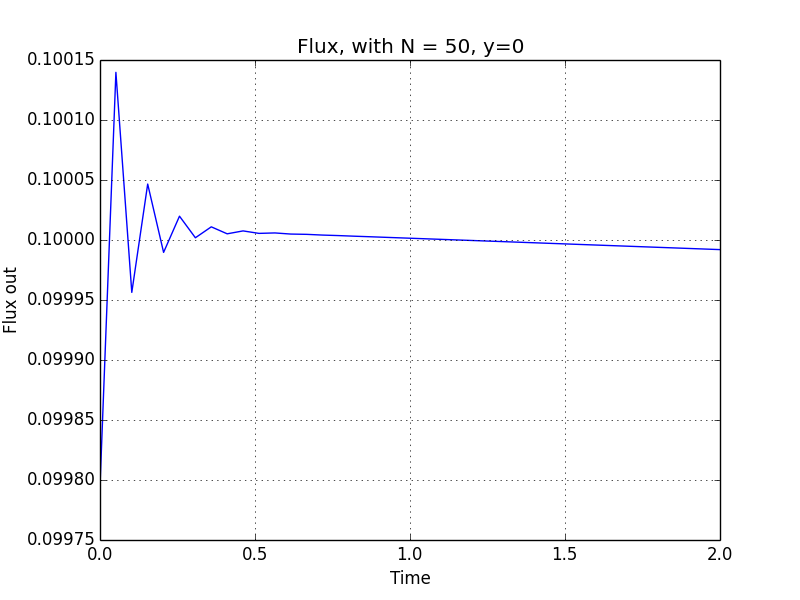
\includegraphics[scale=0.4]{FluxPlot_E_N_50_dt_005.png}



